
\section{ Understandability Estimators}
\label{sec:proxies}
%The previous results highlighted that surface level readability formulas only weakly correlate with human assessments of Web pages understandability (Figure~\ref{fig:bar_corr_clef15}). Next, we considered alternative methods of estimating understandability (Table~\ref{tab:doc_features}), which we present in the following, grouped into categories. 

As reviewed in Section~\ref{sec:related}, several methods have been used to estimate the understandability of health Web pages, with the most popular methods (at least in the biomedical literature) being readability formulas based on surface level characteristics of text. Next, we outline the categories of methods to estimate understandability used in this work; an overview is shown in Table~\ref{tab:doc_features}. Some of these methods further expand measures used in the literature. 
 
%The correlation of readability formulas as shown in Figure~\ref{fig:bar_corr_clef15} %and~\ref{fig:bar_corr_clef16} is not strong, without any correlation coefficient being higher than 0.5.
%Our next intent is comparing the correlation coefficient of the traditional readability formulas with other methods for understandability estimation, including an evaluation of other humans performing the same task.
%For that, we devise and group several methods into semantically related groups which will be following presented. We summarize all methods in Table~\ref{tab:doc_features}.


\textbf{Traditional Readability Formulas (RF):}
These include the readability formulas mentioned in Section~\ref{sec:related}, as well as other, less popular ones. A full list is provided in surveys by Collins-Thompson \cite{collins2014computational} and Dubay~\cite{dubay04}.

%Therefore, what unifies all methods listed in this section is the goal to automatically infer the understandability of a document, in our case, a Web page with medical content.
%For sake of understanding, in Table~\ref{tab:doc_features} we list all the methods used in this chapter to estimate document understandability.
%Note that we divide these estimators into semantically related groups, which are presented below.

%\textbf{Traditional Readability Formulas:}
%This group contains a large set of traditional readability formulas. Some were mentioned in Section~\ref{sec:related}. A full list can be found in surveys such as Collins-Thompson~\cite{collins2014computational} or Dubay~\cite{dubay04}.

\textbf{Raw Components of Readability Formulas (CRF):}
These are formed by the ``building blocks'' used in the traditional readability formulas; examples of such building blocks include the average number of characters per word and the average number of syllables in a sentence. Words are divided into syllables using the Python package Pyphen~\cite{pyphen}.

\textbf{General Medical Vocabularies (GMV):}
These include methods that count the number of words with a medical prefix or suffix, i.e. beginning or ending with Latin or Greek particles (e.g., amni-, angi-, algia-, arteri-), text strings included in lists of acronyms or in medical vocabularies such as the International Statistical Classification of Diseases and Related Health Problems (ICD), Drugbank and the OpenMedSpel dictionary~\cite{openmedspel}. An acronym list from the ADAM database~\cite{zhou2006} is used and methods in this group are matched with documents using simple keywords matching.

\textbf{Consumer Medical Vocabulary (CMV):}
The popular MetaMap \cite{aronson10} tool is used to map the text content of Web pages to entries in  CHV~\cite{zeng06}.
We use the MetaMap semantic types to retain only concepts identified as symptoms or diseases. Similar approaches have been commonly used in the literature (e.g.,~\cite{pang16,agrafiotesA16,palotti16,yates13}).

\textbf{Expert Medical Vocabulary (EMV):}
Similarly to the CHV features, we use MetaMap to convert the content of Web pages into MeSH entities, studying symptoms and disease concepts separately. 

\textbf{Natural Language Features (NLF):}
These include commonly used natural language heuristics such as the ratio of part-of-speech (POS) classes, the number of entities in the text, the sentiment polarity and the ratio of words found in English vocabularies. The Python package NLTK~\cite{nltk} is employed for sentiment analysis and POS tagging. The GNU Aspell~\cite{aspell} dictionary is used as a standard English vocabulary and a stop word list is built by merging those of Indri~\cite{indri} and Terrier~\cite{terrier}. 

\textbf{HTML Features (HF):}
These include the identification of a large number of HTML tags, which are extracted with the Python library BeautifulSoap~\cite{bs4}. The intuition for these features is that Web pages with many images and tables may explain and summarise health content better, thus providing more understandable content to the general public. 

\textbf{Word Frequency Features (WFF):}
Generally speaking, common and known words are usually frequent words, while unknown and obscure words are generally rare. This idea is implemented in readability formulas such as the DCI, which uses a list of common words and counts the number of words that fall outside this list (complex words)~\cite{dale48}.
We extend these observations by studying corpus-wide word frequencies. 
We model word frequencies in a corpus in a straightforward manner: we sort the word frequencies and normalize word rankings such that values close to 100 are attributed to common words and values close to 0 to rare words. Three corpora are analysed to extract word frequencies:

\begin{itemize}[leftmargin=*]
\item \underline{Medical Reddit:} Reddit~\cite{reddit} is a Web forum with a sizeable user community which is responsible for generating and moderating its content. Any user can start a discussion or reply to a discussion. This forum is intensively used for health purposes, for example in the Reddit community AskDocs~\cite{redditaskdocs}, licensed nurses and doctors (subject to user identity verification) advise help seekers free of charge. We selected six of such communities
    (medical, AskDocs, AskDoctorSmeeee, Health, WomensHealth, Mens\_Health) and downloaded all user interactions available until September 1st 2017 using the Python library PRAW~\cite{redditapi}. In total 43,018 discussions were collected.

\item \underline{Medical English Wikipedia:} after obtaining a recent  Wikipedia dump~\cite{wikipedia} (May 1st 2017), we filtered articles to only those  containing an Infobox\footnote{A Wikipedia infobox is a structured template that appears on the right of Wikipedia pages summarizing key aspects of articles.} in which at least one of the following words appeared as a property: ICD10, ICD9, DiseasesDB, MeSH, MeSHID, MeshName, MeshNumber, GeneReviewsName, Orphanet, eMedicine, MedlinePlus, drug\_name, Drugs.com, DailyMedID, LOINC.
%Figure~\ref{fig:hyperthermia} illustrates a Wikipedia page that is marked as medical because of its Infobox entries.
In doing so, we followed the method by Soldaini et al.~\cite{soldaini15}, which favours precision over recall when identifying a health-related article. This resulted in a collection of 11,942 articles. 
%Note that this procedure highly favors precision over recall. %\mytodo{In case we need space, I suggest we drop this figure}

\item \underline{PubMed Central:} PubMed Central~\cite{pubmed} is an online  database of freely available full-text biomedical literature. We used the same collection distributed for the TREC 2014 and 2015 Clinical Decision Support Track~\cite{roberts16,trec15}, consisting of 733,138 articles. 
 
\end{itemize}

A summary of the statistics of these three collections is reported in Table~\ref{tab:collection_stats}. 
%We removed words that occurred less than 5 times in a corpus.  %% We include this detail if necessary in the final version of this paper
Finally, unless explicitly stated otherwise, we ignored out of vocabulary words in our feature calculations.



%\begin{figure}[th!]
%   \centering
%   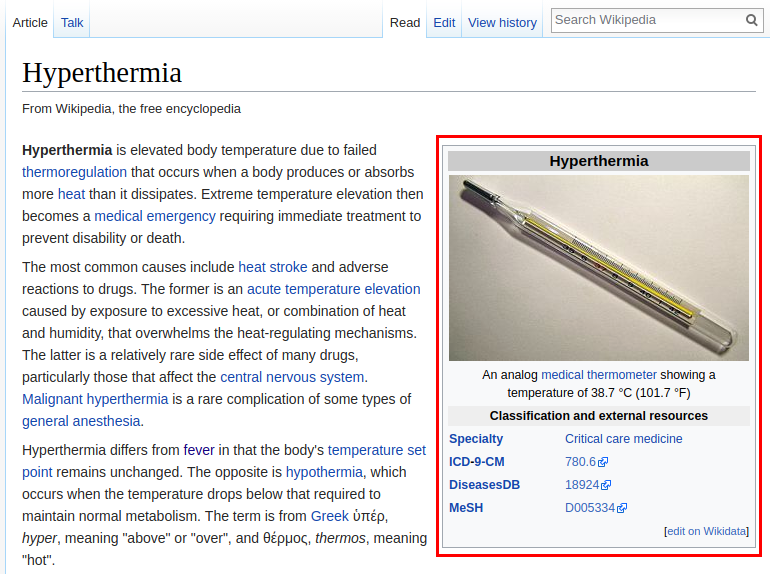
\includegraphics[width=0.50\textwidth]{graphics/hyperthermia}
%    \caption{Wikipedia page on hyperthermia. A rectangular red box identify the Infobox on the right hand side containing entries for Specialty, ICD-9-CM, DiseasesDB and MeSH.}
%    \label{fig:hyperthermia}
%\end{figure}

\begin{table}[!tb]
\centering    
\caption{Statistics for the collections used as background models for understandability estimations.}
\vspace{-0.3cm}
\label{tab:collection_stats}
\resizebox{0.4\textwidth}{!}{
\begin{tabular}{cccc}
\toprule 
\textbf{Statistic} & \textbf{Medical Wikipedia} & \textbf{Medical Reddit} & \textbf{PubMed Central}\tabularnewline
\midrule 
\textbf{Number of Docs.} & 11,868 & 43,019 & 733,191\tabularnewline
\textbf{Number of Words} & 10,655,572 & 11,978,447 & 144,024,976\tabularnewline
\textbf{Number of Unique Words} & 467,650 & 317,106 & 2,933,167\tabularnewline
\textbf{Avg. Words per Doc.} & 898.90 $\pm$ 1351.76 & 278.45 $\pm$ 359.70  & 227.22 $\pm$ 270.44 \tabularnewline
\textbf{Avg. Char per Doc.} & 5107.81 $\pm$ 7618.57  & 1258.44 $\pm$ 1659.96  & 1309.11 $\pm$ 1447.31 \tabularnewline
\textbf{Avg. Char per Word} & 5.68 $\pm$ 3.75  & 4.52 $\pm$ 3.52 &  5.76 $\pm$ 3.51 \tabularnewline
\bottomrule
\end{tabular}
} % End of resizebox
\vspace{-8pt}
\end{table}


\textbf{Machine Learning on Text - Regressors (MLR) and Classifiers (MLC):} These include machine learning methods for estimating Web page understandability. While Collins-Thompson highlighted the promise of estimating understandability using machine learning methods, a challenge is identifying the background corpus to be used for training~\cite{collins2014computational}. To this aim, we use the three corpora detailed above, and assume understandability labels according to the expected difficulty of documents in these collections:

\begin{itemize}[leftmargin=*]
    \item Medical Reddit (label 1): Documents in this collection are expected to be written in a colloquial style, and thus the easiest to understand. All the conversations are in fact explicitly directed to assist inexpert health consumers;
    \item Medical English Wikipedia (label 2): Documents in this collection are expected to be less formal than scientific articles, but more formal than a Web forum like Reddit, thus somewhat more difficult to understand;
    \item PubMed Central (label 3): Documents from this collection are expected to be written in a highly formal style, as the target audience are physicians and biomedical researchers.
\end{itemize}

Models are learned using all documents from these collections after features are extracted using Latent Semantic Analysis (LSA) with 10 dimensions (empirically set based on document word counts in the three collections). We model a classification task as well as a regression task using these collections. Thus, after applying the same LSA transformation to test documents from CLEF, a continuous score is assigned to each document by a regressor\footnote{In principal the regressors should output a continuous value between 1 and 3, but no restrictions are set and potentially any value can be assigned to a document.}, while each classifier assigns the documents to one of the three classes.

%Different labels for the regression could be employed, for example, a label 6 to PubMed Central documents would emphasize that these documents are explicitly made for expert users, being 3 times harder than Wikipedia ones. We did not explore the effects of different labels in this work, it is left as future work.

\begin{table*}[tb]
\caption{Metrics used as understandability proxies; $\star$: raw values are used. $\diamondsuit$: values normalised by number of words in a documents are used. $\dagger$: values normalised by number of sentences in a document are used.}
\label{tab:doc_features}
\resizebox{1.\textwidth}{!}{
\begin{tabular}{llcll}
\cline{1-2} \cline{4-5} 
\textbf{Group} & \textbf{Metric} & \multirow{29}{*}{} & \textbf{Group} & \textbf{Metric}\tabularnewline
\cline{1-2} \cline{4-5} 
\multirow{8}{*}{\textbf{Traditional Readability Formulas}} & Automated Readability Index (ARI) \cite{ari67} &  & \multirow{26}{*}{\textbf{HTML Features}} & \# of Abbr tags\tabularnewline
 & Coleman-Liau Index (CLI) \cite{cli75} &  &  & \# of A tags\tabularnewline
 & Dale Chall Index (DCI) \cite{dale48} &  &  & \# of Blockquote tags\tabularnewline
 & Flesch-Kincaid Grade Level (FKGL) \cite{flesch75} &  &  & \# of Bold tags\tabularnewline
 & Flesch Reading Ease (FRE) \cite{flesch75} &  &  & \# of Cite tags\tabularnewline
 & Gunning Fog Index (GFI) \cite{gunning52} &  &  & \# of Div tags\tabularnewline
 & Lasbarhetsindex (LIX) \cite{lix} &  &  & \# of Forms tags\tabularnewline
 & Simple Measure of Gobbledygook (SMOG) \cite{smog69} &  &  & \# of H1 tags\tabularnewline
\cline{1-2} 
\multirow{10}{*}{\textbf{\makecell{\kern-2.8emRaw Components \\of Readability Measures}}} & \# of Characters $^{\star\diamondsuit\dagger}$ &  &  & \# of H2 tags\tabularnewline
 & \# of Words $^{\star\dagger}$ &  &  & \# of H3 tags\tabularnewline
 & \# of Sentences {$^{\star\diamondsuit}$} &  &  & \# of H4 tags\tabularnewline
 & \# of Difficult Words (Dale Chall list \cite{dale48})
$^{\star\diamondsuit\dagger}$ &  &  & \# of H5 tags\tabularnewline
 & \# of Words Longer than 4 chars $^{\star\diamondsuit\dagger}$ &  &  & \# of H6 tags\tabularnewline
 & \# of Words Longer than 6 chars $^{\star\diamondsuit\dagger}$ &  &  & \# of Hs (any H above)\tabularnewline
 & \# of Words Longer than 10 chars $^{\star\diamondsuit\dagger}$ &  &  & \# of Img tags\tabularnewline
 & \# of Words Longer than 13 chars $^{\star\diamondsuit\dagger}$ &  &  & \# of Input tags\tabularnewline
 & \# of Number of Syllables $^{\star\diamondsuit\dagger}$ &  &  & \# of Link tags\tabularnewline
 & \# of Polysyllable Words (>3 Syllables) $^{\star\diamondsuit\dagger}$ &  &  & \# of DL tags\tabularnewline
\cline{1-2} 
\multirow{6}{*}{\textbf{Medical Vocabularies}} & \# of Words with Medical Prefix $^{\star\diamondsuit\dagger}$ &  &  & \# of UL tags\tabularnewline
 & \# of Words with Medical Suffix $^{\star\diamondsuit\dagger}$ &  &  & \# of OL tags\tabularnewline
 & \# of Acronyms $^{\star\diamondsuit\dagger}$ &  &  & \# of List (DL + UL + OL)\tabularnewline
 & \# of ICD Concepts $^{\star\diamondsuit\dagger}$ &  &  & \# of Q tags\tabularnewline
 & \# of Drugbank $^{\star\diamondsuit\dagger}$ &  &  & \# of Scripts tags\tabularnewline
 & \# of Words in medical dict. (OpenMedSpel) $^{\star\diamondsuit\dagger}$ &  &  & \# of Spans tags\tabularnewline
\cline{1-2} 
    \multirow{6}{*}{\textbf{\makecell{\kern-2.5emConsumer Health\\ Vocabulary (CHV) \cite{zeng06} \\ \kern-6.2emFeatures}}} & CHV Mean Score for all Concepts $^{\star\diamondsuit\dagger}$ &  &  & \# of Table tags\tabularnewline
 & \# of CHV Concepts $^{\star\diamondsuit\dagger}$ &  &  & \# of P tags\tabularnewline
\cline{4-5} 
 & CHV Mean Score for Symptom Concepts $^{\star\diamondsuit\dagger}$ &  & \multirow{20}{*}{\textbf{Word Frequency}} & 25th percentil English Wikipedia\tabularnewline
 & \# of CHV Symptom Concepts $^{\star\diamondsuit\dagger}$ &  &  & 50th percentil English Wikipedia\tabularnewline
 & CHV Mean Score for Disease Concepts $^{\star\diamondsuit\dagger}$ &  &  & 75th percentil English Wikipedia\tabularnewline
 & \# of CHV Disease Concepts $^{\star\diamondsuit\dagger}$ &  &  & Mean Rank English Wikipedia\tabularnewline
\cline{1-2} 
\multirow{6}{*}{\textbf{\makecell{\kern-0.3emMedical Subject\\ Headers (MeSH)}}} & \# of MeSH Concepts $^{\star\diamondsuit\dagger}$ &  &  & Mean Rank English Wikipedia - Includes OV\tabularnewline
 & Average Tree of MeSH Concepts $^{\star\diamondsuit\dagger}$ &  &  & 25th percentil Medical Reddit\tabularnewline
 & \# of MeSH Symptom Concepts $^{\star\diamondsuit\dagger}$ &  &  & 50th percentil Medical Reddit\tabularnewline
 & Average Tree of MeSH Symptom Concepts $^{\star\diamondsuit\dagger}$ &  &  & 75th percentil Medical Reddit\tabularnewline
 & \# of MeSH Disease Concepts $^{\star\diamondsuit\dagger}$ &  &  & Mean Rank Medical Reddit\tabularnewline
 & Average Tree of MeSH Disease Concepts $^{\star\diamondsuit\dagger}$ &  &  & Mean Rank Medical Reddit ncludelude OV\tabularnewline
\cline{1-2} 
\multirow{20}{*}{\textbf{Natural Language}} & Positive Words $^{\star\diamondsuit\dagger}$ &  &  & 25th percentil Pubmed\tabularnewline
 & Negative Words $^{\star\diamondsuit\dagger}$ &  &  & 50th percentil Pubmed\tabularnewline
 & Neutral Words $^{\star\diamondsuit\dagger}$ &  &  & 75th percentil Pubmed\tabularnewline
 & \# of verbs $^{\star\diamondsuit\dagger}$ &  &  & Mean Rank Pubmed\tabularnewline
 & \# of nouns $^{\star\diamondsuit\dagger}$ &  &  &  Mean Rank Pubmed - Includes OV\tabularnewline
 & \# of pronouns $^{\star\diamondsuit\dagger}$ &  &  & 25th p. Wikipedia+Reddit+Pubmed  \tabularnewline
 & \# of adjectives $^{\star\diamondsuit\dagger}$ &  &  & 50th p. Wikipedia+Reddit+Pubmed \tabularnewline
 & \# of adverbs $^{\star\diamondsuit\dagger}$ &  &  & 75th p. Wikipedia+Reddit+Pubmed \tabularnewline
 & \# of adpositions $^{\star\diamondsuit\dagger}$ &  &  & Mean R. Wiki.+Reddit+Pubmed \tabularnewline 
 & \# of conjunctions $^{\star\diamondsuit\dagger}$ & &  & Mean R. Wiki.+Reddit+Pubmed - w. OV \tabularnewline
\cline{4-5} 
 & \# of determiners $^{\star\diamondsuit\dagger}$ & & \multirow{5}{*}{\textbf{Regressor}} & Linear Regressor\tabularnewline  
 & \# of cardinal numbers $^{\star\diamondsuit\dagger}$ &  &  & Gradient Boosting Regressor\tabularnewline
 & \# of particles or other function words $^{\star\diamondsuit\dagger}$ &  &  & Multi-layer Perceptron Regressor\tabularnewline
 & \# of other POS (foreign words, typos) $^{\star\diamondsuit\dagger}$ &  &  & Random Forest Regressor\tabularnewline
 & \# of punctuation $^{\star\diamondsuit\dagger}$ &  &  & Support Vector Machine Regressor\tabularnewline
\cline{4-5} 
 & Height of part-of-speech parser tree $^{\star\diamondsuit\dagger}$ &  &  \multirow{6}{*}{\textbf{Classifier}} & Logistic Regression\tabularnewline
 & \# of Entities $^{\star\diamondsuit\dagger}$ &  &  & Gradient Boosting Classifier\tabularnewline
 & \# of Stopwords $^{\star\diamondsuit\dagger}$ &  &  & Multinomial Naive Bayes\tabularnewline
 & \# of words not found in Aspell Eng. dict. $^{\star\diamondsuit\dagger}$ &  &  & Multi-layer Perceptron Classifier\tabularnewline
 &  &  &  & Random Forest Classifier\tabularnewline
 &  &  &  & Support Vector Machine Classifier\tabularnewline
\cline{1-2} \cline{4-5} 
\end{tabular}
}
\end{table*}



